\documentclass[aspectratio=169]{beamer}
\PassOptionsToPackage{english}{babel}
\usepackage{standardslides}

\def\UrlBigBreaks{\do\/\do-\do:}

\title{Design and Implementation of Vectorized Pseudorandom Number Generators and their Application to Simulations of Photon Propagation}
\author{Markus Pawellek}

\begin{document}
  \selectlanguage{english}
  % \urlstyle{sf}

  \frame{\titlepage}
  \begin{frame}{Outline}
    \footnotesize
    \hfill\parbox[t][7cm][l]{0.9\textwidth}{\tableofcontents}
  \end{frame}

  \section{Introduction and Motivation} % (fold)
  \label{sec:introduction_and_motivation}
    \begin{frame}{Preliminaries}
      \begin{itemize}
        \item no c++ code shown
        \item why c++
        \item only two generators
        \item a few things will not be shown
        \item no theory shown why prngs good

      \end{itemize}
    \end{frame}

    \begin{frame}{Monte-Carlo Methods and Physical Simulations}

    \end{frame}

    \begin{frame}{Computation of π}
      \begin{figure}
        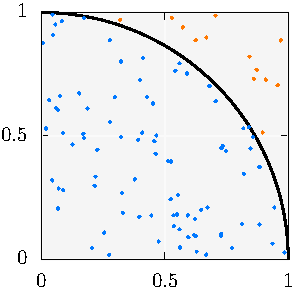
\includegraphics[width=0.3\textwidth]{figures/monte_carlo_pi_100_87.pdf}
        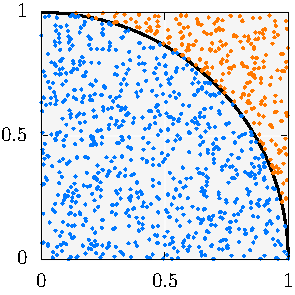
\includegraphics[width=0.3\textwidth]{figures/monte_carlo_pi_1000_765.pdf}
        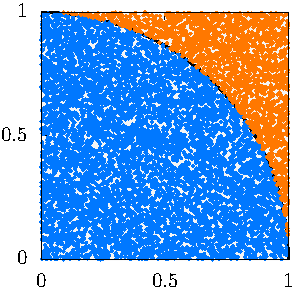
\includegraphics[width=0.3\textwidth]{figures/monte_carlo_pi_10000_7856.pdf}
      \end{figure}
    \end{frame}
  % section introduction_and_motivation (end)

  \section{Pseudorandom Number Generators} % (fold)
  \label{sec:pseudorandom_number_generators}
    \begin{frame}{Concepts}
      \begin{figure}
        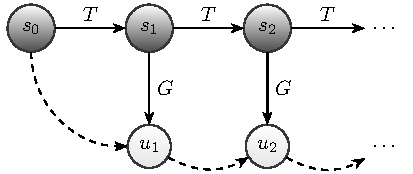
\includegraphics[width=0.5\textwidth]{figures/sequence_generation_scheme.pdf}
      \end{figure}
    \end{frame}

    \begin{frame}{Mersenne Twister MT19937}
      \begin{figure}
        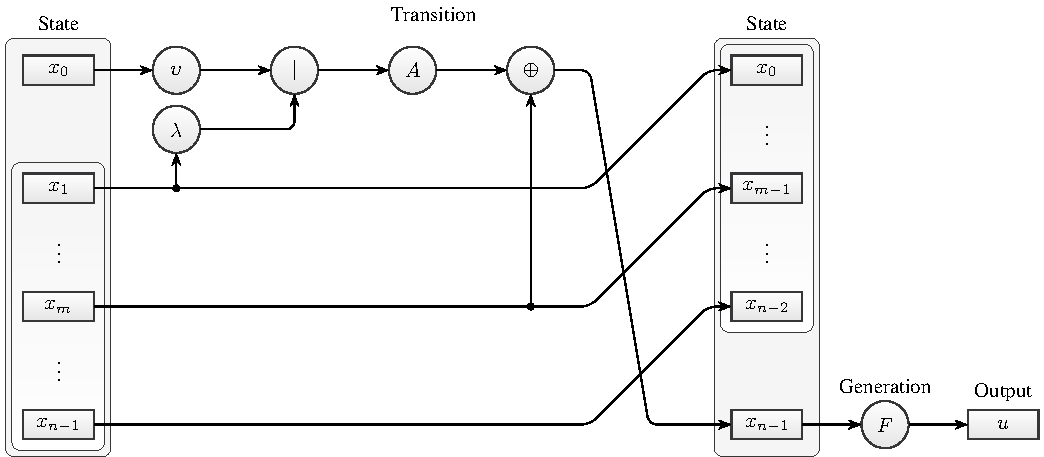
\includegraphics[width=0.8\textwidth]{figures/mt19937_scheme.pdf}
      \end{figure}
    \end{frame}

    \begin{frame}{Xoroshiro128+}
      \begin{figure}
        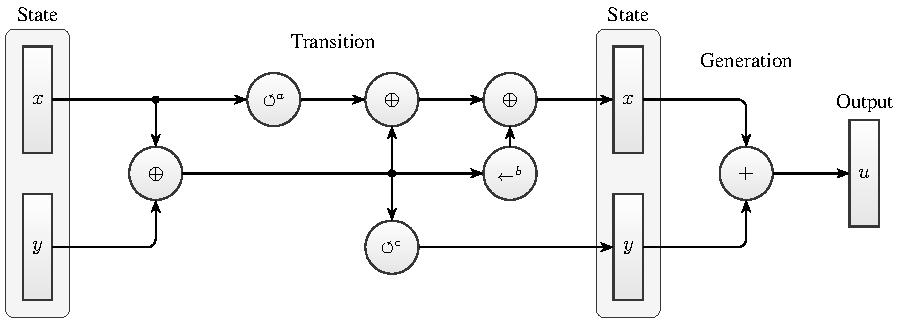
\includegraphics[width=0.8\textwidth]{figures/xrsr128p_scheme.pdf}
      \end{figure}
    \end{frame}
  % section pseudorandom_number_generators (end)

  \section{Fundamentals of Computer Architecture} % (fold)
  \label{sec:fundamentals_of_computer_architecture}
    \begin{frame}{Processor and Memory}
      \begin{figure}
        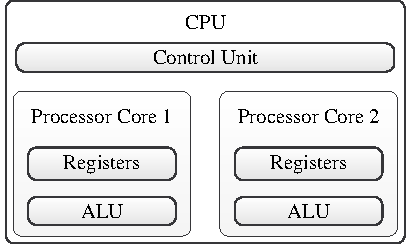
\includegraphics[height=0.5\textheight]{figures/cpu_components.pdf}
      \end{figure}
    \end{frame}

    \begin{frame}{Memory Hierarchy}
      \begin{figure}
        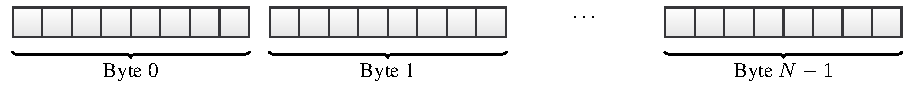
\includegraphics[width=0.95\textwidth]{figures/memory.pdf}
      \end{figure}
      \begin{figure}
        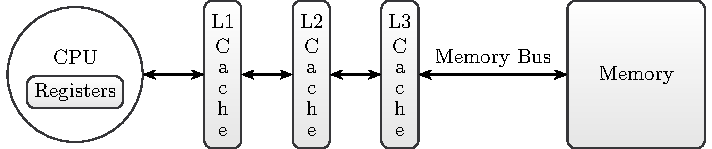
\includegraphics[width=0.95\textwidth]{figures/memory_hierarchy.pdf}
      \end{figure}
    \end{frame}

    \begin{frame}{SIMD and Intrinsics}
      \begin{figure}
        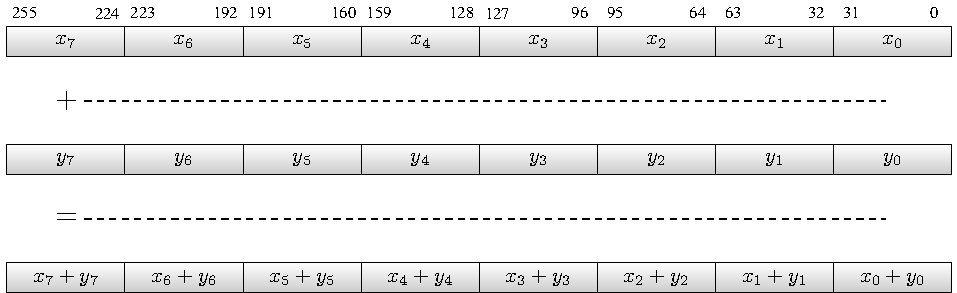
\includegraphics[width=0.95\textwidth]{figures/simd_vector_operations.pdf}
      \end{figure}
    \end{frame}

    \begin{frame}{Uniform Floating-Point Numbers}
      \begin{figure}
        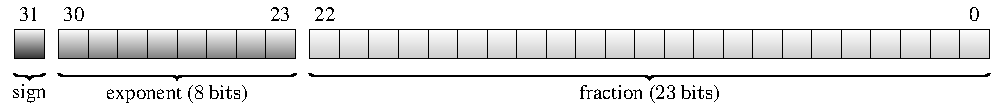
\includegraphics[width=0.95\textwidth]{figures/floating-point_encoding_single.pdf}
      \end{figure}
      \begin{figure}
        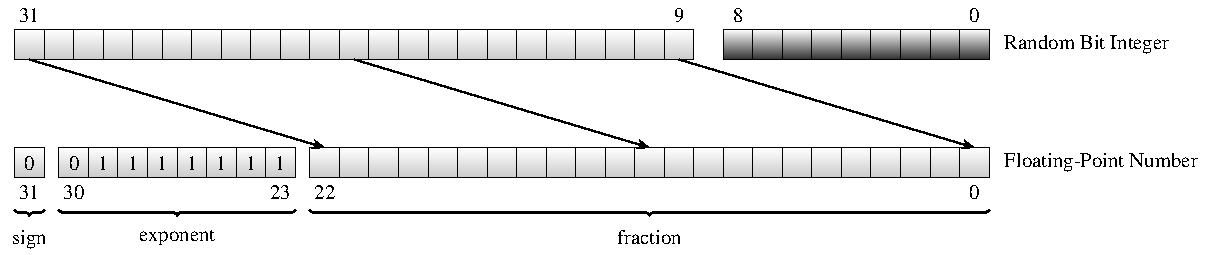
\includegraphics[width=0.95\textwidth]{figures/uniform_implementation_scheme.pdf}
      \end{figure}
    \end{frame}
  % section fundamentals_of_computer_architecture (end)

  \section{Design} % (fold)
  \label{sec:design}
    \begin{frame}{C++ Design Concepts for Libraries}

    \end{frame}
  % section design (end)

  \section{Implementation} % (fold)
  \label{sec:implementation}
    \begin{frame}{Xoroshiro128+ Scalar and Vectorized}
      \begin{figure}
        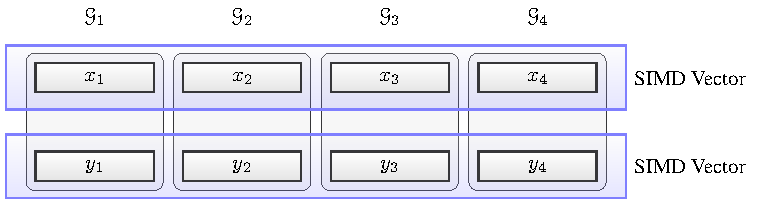
\includegraphics[width=0.9\textwidth]{figures/xrsr128p_vector_layout.pdf}
      \end{figure}
    \end{frame}

    \begin{frame}{MT19937 Scalar and Vectorized}
      \begin{figure}
        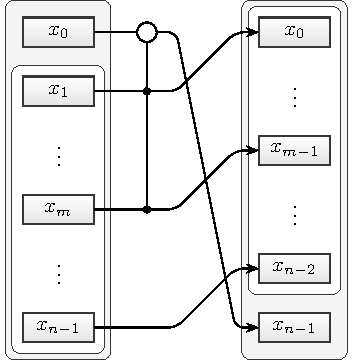
\includegraphics[width=0.25\textwidth]{figures/mt19937_transition_short.pdf}
        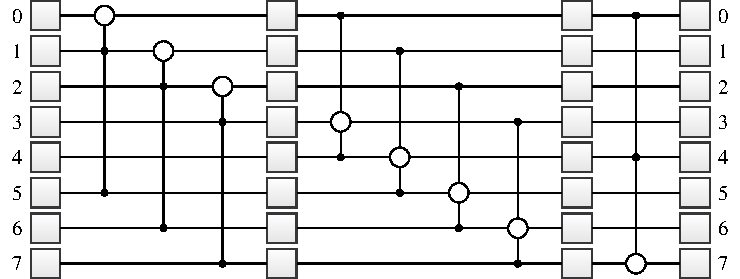
\includegraphics[width=0.7\textwidth]{figures/mt19937_loop_scheme.pdf}
      \end{figure}
    \end{frame}

    \begin{frame}{MT19937 SIMD}
      \begin{figure}
        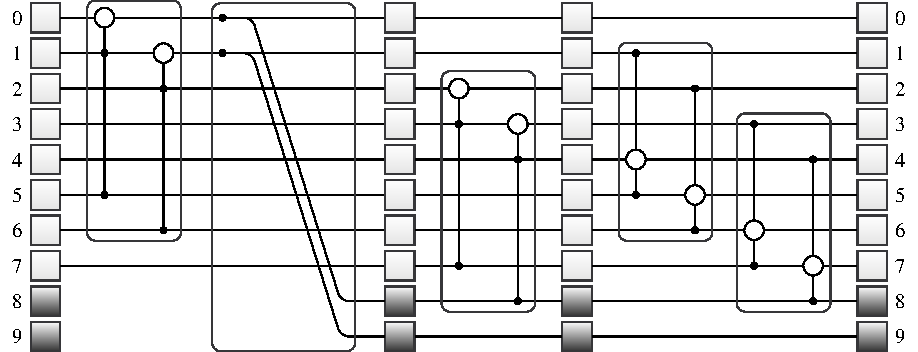
\includegraphics[width=0.9\textwidth]{figures/mt19937_vector_loop_scheme.pdf}
      \end{figure}
    \end{frame}
  % section implementation (end)

  \section{Tests and Benchmarks} % (fold)
  \label{sec:tests_and_benchmarks}
    \begin{frame}{Statistical Performance}

    \end{frame}

    \begin{frame}{API Tests}

    \end{frame}

    \begin{frame}{Photon Simulation}

    \end{frame}

    \begin{frame}{Previous Work}

    \end{frame}
  % section tests_and_benchmarks (end)

  \section{Evaluation and Results} % (fold)
  \label{sec:evaluation_and_results}
    \begin{frame}{Evaluation and Results}
      \begin{figure}
        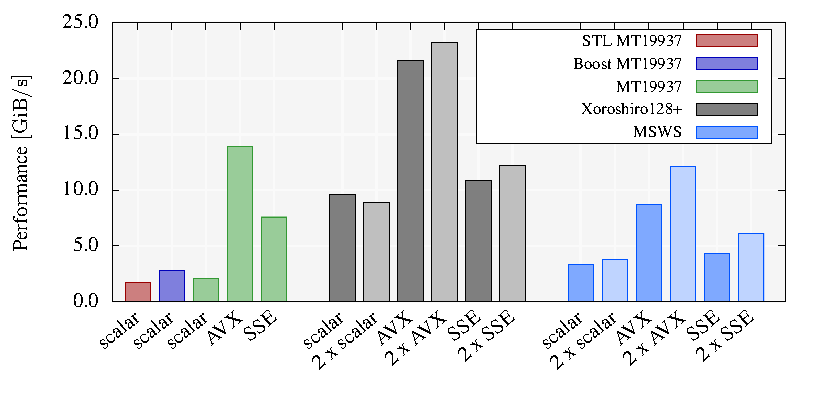
\includegraphics[width=0.6\textwidth]{figures/generation_desktop.pdf}
      \end{figure}
    \end{frame}

    \begin{frame}
      \begin{figure}
        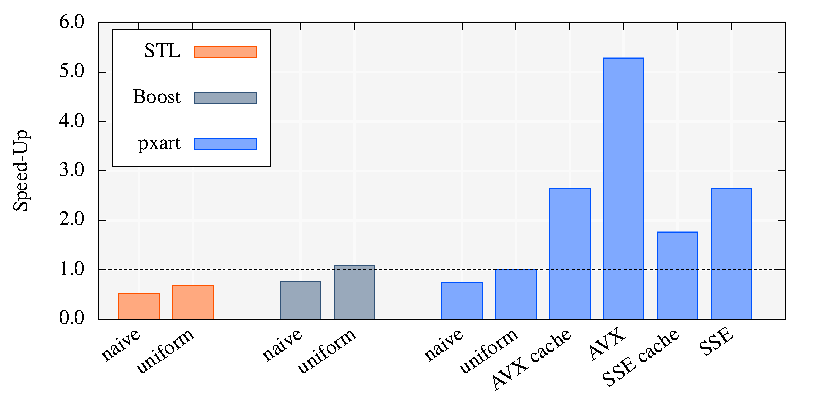
\includegraphics[width=0.6\textwidth]{figures/monte_carlo_pi_desktop_mt19937.pdf}\\
        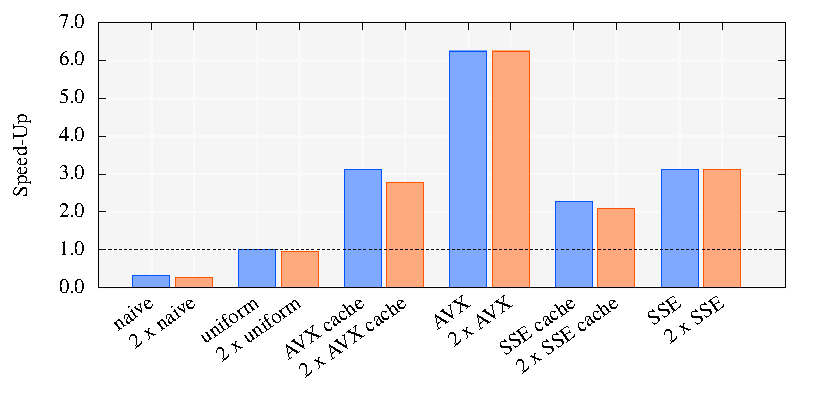
\includegraphics[width=0.6\textwidth]{figures/monte_carlo_pi_desktop_xrsr128p.pdf}
      \end{figure}
    \end{frame}
  % section evaluation_and_results (end)

  \section{Conclusions and Future Work} % (fold)
  \label{sec:conclusions}
    \begin{frame}{Conclusions and Future Work}
      \begin{itemize}
        \item possible applications in simulations
        \item mt19937 vs. xoroshiro128+
      \end{itemize}
    \end{frame}
  % section conclusions (end)

  \begin{frame}
    \frametitle{References}
    % \tiny
    % \begin{multicols}{2}
    %   \nocite{*}
    %   \bibliography{references}
    % \end{multicols}
  \end{frame}
\end{document}